\documentclass{article}
% Include all project wide packages here.
\usepackage{fullpage}
\usepackage[style=ieee]{biblatex}
\usepackage[dutch]{babel}

\renewcommand{\familydefault}{\sfdefault}

\setmainfont[Ligatures=TeX]{Myriad Pro}
\setmathfont{Asana Math}
\setmonofont{Lucida Console}

\usepackage{titlesec, blindtext, color}
\definecolor{gray75}{gray}{0.75}
\newcommand{\hsp}{\hspace{20pt}}
\titleformat{\chapter}[hang]{\Huge\bfseries}{\thechapter\hsp\textcolor{gray75}{|}\hsp}{0pt}{\Huge\bfseries}
\renewcommand{\familydefault}{\sfdefault}
\renewcommand{\arraystretch}{1.2}
\setlength\parindent{0pt}

%For code listings
\definecolor{black}{rgb}{0,0,0}
\definecolor{browntags}{rgb}{0.65,0.1,0.1}
\definecolor{bluestrings}{rgb}{0,0,1}
\definecolor{graycomments}{rgb}{0.4,0.4,0.4}
\definecolor{redkeywords}{rgb}{1,0,0}
\definecolor{bluekeywords}{rgb}{0.13,0.13,0.8}
\definecolor{greencomments}{rgb}{0,0.5,0}
\definecolor{redstrings}{rgb}{0.9,0,0}
\definecolor{purpleidentifiers}{rgb}{0.01,0,0.01}


\lstdefinestyle{csharp}{
language=[Sharp]C,
showspaces=false,
showtabs=false,
breaklines=true,
showstringspaces=false,
breakatwhitespace=true,
escapeinside={(*@}{@*)},
columns=fullflexible,
commentstyle=\color{greencomments},
keywordstyle=\color{bluekeywords}\bfseries,
stringstyle=\color{redstrings},
identifierstyle=\color{purpleidentifiers},
basicstyle=\ttfamily\small}

\lstdefinestyle{c}{
language=C,
showspaces=false,
showtabs=false,
breaklines=true,
showstringspaces=false,
breakatwhitespace=true,
escapeinside={(*@}{@*)},
columns=fullflexible,
commentstyle=\color{greencomments},
keywordstyle=\color{bluekeywords}\bfseries,
stringstyle=\color{bluestrings},
identifierstyle=\color{purpleidentifiers}
}

\lstdefinestyle{vhdl}{
language=VHDL,
showspaces=false,
showtabs=false,
breaklines=true,
showstringspaces=false,
breakatwhitespace=true,
escapeinside={(*@}{@*)},
columns=fullflexible,
commentstyle=\color{greencomments},
keywordstyle=\color{bluekeywords}\bfseries,
stringstyle=\color{redstrings},
identifierstyle=\color{purpleidentifiers}
}

\lstdefinestyle{xaml}{
language=XML,
showspaces=false,
showtabs=false,
breaklines=true,
showstringspaces=false,
breakatwhitespace=true,
escapeinside={(*@}{@*)},
columns=fullflexible,
commentstyle=\color{greencomments},
keywordstyle=\color{redkeywords},
stringstyle=\color{bluestrings},
tagstyle=\color{browntags},
morestring=[b]",
  morecomment=[s]{<?}{?>},
  morekeywords={xmlns,version,typex:AsyncRecords,x:Arguments,x:Boolean,x:Byte,x:Char,x:Class,x:ClassAttributes,x:ClassModifier,x:Code,x:ConnectionId,x:Decimal,x:Double,x:FactoryMethod,x:FieldModifier,x:Int16,x:Int32,x:Int64,x:Key,x:Members,x:Name,x:Object,x:Property,x:Shared,x:Single,x:String,x:Subclass,x:SynchronousMode,x:TimeSpan,x:TypeArguments,x:Uid,x:Uri,x:XData,Grid.Column,Grid.ColumnSpan,Click,ClipToBounds,Content,DropDownOpened,FontSize,Foreground,Header,Height,HorizontalAlignment,HorizontalContentAlignment,IsCancel,IsDefault,IsEnabled,IsSelected,Margin,MinHeight,MinWidth,Padding,SnapsToDevicePixels,Target,TextWrapping,Title,VerticalAlignment,VerticalContentAlignment,Width,WindowStartupLocation,Binding,Mode,OneWay,xmlns:x}
}

%defaults
\lstset{
basicstyle=\ttfamily\small,
extendedchars=false,
numbers=left,
numberstyle=\ttfamily\tiny,
stepnumber=1,
tabsize=4,
numbersep=5pt
}
\addbibresource{../../library/bibliography.bib}

\title{Niet lineaire schakelingen: versterking met een BPT}
\author{Robin Hes; Chy Lau; Tijmen Witte}
\begin{document}
\maketitle

\section*{Inleiding}

Tijdens de Just-in-time training van 24-04-2013 was het bedoeling dat we meer inzicht zouden krijgen in niet-lineaire elektronische componenten. Hierdoor 
zijn we beter voorbereid om een ontwerp te maken voor een mogelijke mijndetecterende sensor voor de robot. Bij deze opdrachten zouden we gebruik maken van verschillende simulatieprogramma's (Falstad en SPICE) om een eerste schatting van bepaalde waarden te verkrijgen en vervolgens om een precies gedrag van componenten te verkrijgen.

\begin{figure}[H]
	\centering
	\label{fig:npn-amplifier}
	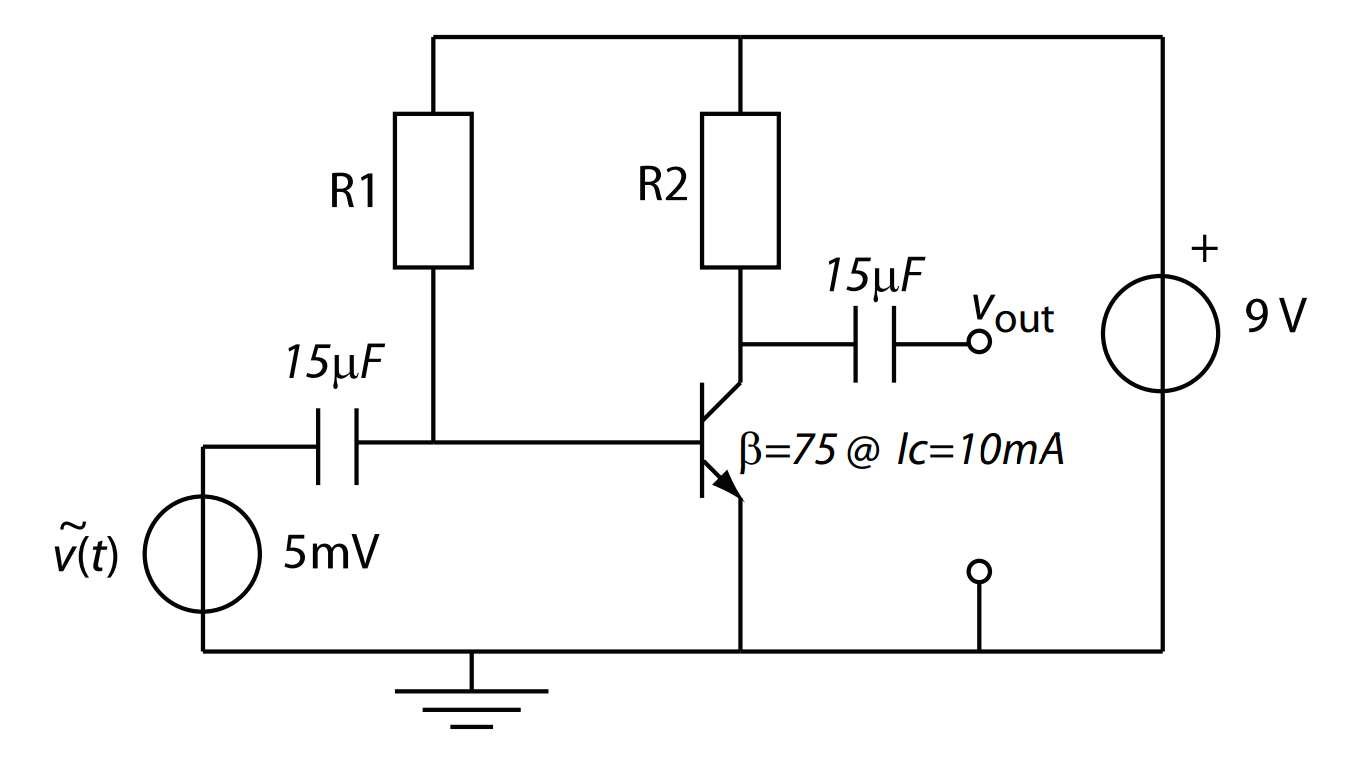
\includegraphics[width=0.6\textwidth]{resource/npn-amplifier}
	\caption{Spanningsversterker op basis van een bipolaire NPN-transistor \cite[p.~3]{epo2-non-linear}}
\end{figure}

\noindent
In dit verslag behandelen we een versterker op basis van een bipolaire NPN-transistor met een terugkoppelcircuit van twee weerstanden. Als eerste bepalen we geschikte waarden voor de twee weerstanden, vervolgens komt het groot-signaal model aan bod en als laatst bespreken we het klein-signaal model.

\section*{Weerstandswaarden $R_1$, $R_2$}

\begin{equation}
\frac{V_{CC}-V_{BE}}{R_1}=I_B 
\end{equation}
$$\Rightarrow R_1=\frac{V_{CC}-V_{BE}}{I_B}$$

\noindent De basisstroom wordt berekend door de collectorstroom te delen met de versterkingsfactor van de transistor,

\begin{equation}
I_C=I_B \cdot \beta
\end{equation}
$$\Rightarrow I_B=\frac{I_C}{\beta}$$
$$\Rightarrow I_B=\frac{10 \: mA}{75}=1.3\times 10^{-4}A$$

\noindent Alle waarden in formule 1 invullen geeft,
$$\Rightarrow R_1=\frac{9\: V-0.7\: V}{1.3\times 10^{-4}A}$$
$$\Rightarrow R_1=63.8 \: k  \Omega$$

\noindent Om de waarden van $R_2$ te berekenen, veronderstellen we dat de collector spanning $V_C$ gelijk is aan 4.5 V. Een spanning van 4.5 V geeft het meeste bereik naar de aarde en naar de voedingsspanning $V_{CC}$ van 9 V. 

\begin{equation}
V = I \cdot R 
\end{equation}

$$R_2 = \frac{V_{CC}-V_C}{I_C} = \frac{9\:V-4.5\:V}{10\:mA}=450\: \Omega$$

\section*{Groot-signaal model en instelpunt}

Het groot-signaal equivalent circuit maakt het mogelijk om de niet-lineaire schakeling te beschrijven. De spanning die wordt aangeboden aan de ingang is een sinusvormig signaal en kan al bij grotere waarden ertoe leiden dat de uitgangsspanning geen lineaire versterking is van de ingangsspanning.

\begin{figure}[H]
	\centering
	\label{fig:npn-amplifier-grootsignaal}
	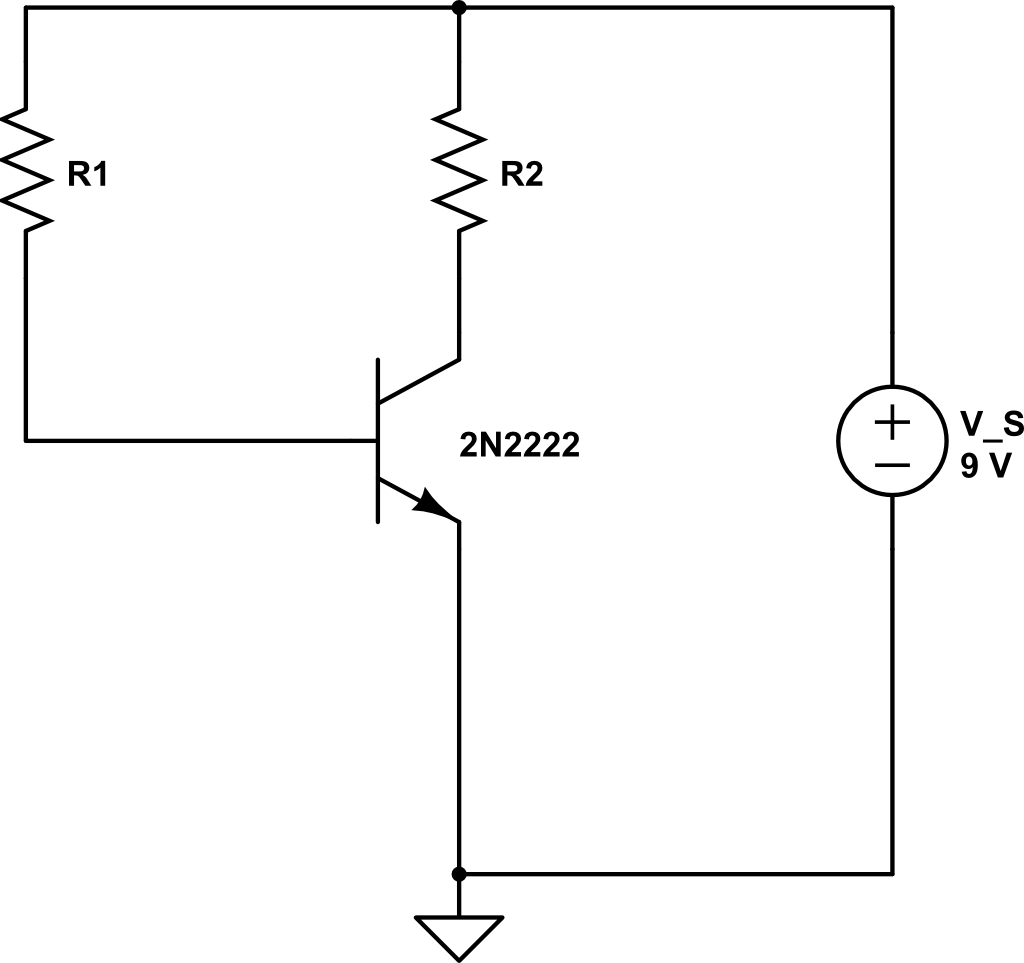
\includegraphics[width=0.4\textwidth]{resource/npn-grootsignaal-versterker}
	\caption{Grootsignaalmodel van NPN-spanningsversterker}
\end{figure}

De versterkingsfactor van de 2N2222 transistor is 75 \cite[p.~3]{epo2-non-linear}. Als er een bepaalde ingangsspanning wordt geleverd, kan het zo zijn dat de voedingsspanning van 9 V de versterking niet kan leveren. Hierdoor ontstaat er niet een sinusgrafiek met een grotere amplitude, maar bijvoorbeeld een blokgolf (de uitgangsspanning wordt geclipt).\\

Het instelpunt (operating point) is het punt waarbij de uitgangsspanning ongeveer de helft is van de voedingsspanning bij een geen-ingangsspanning conditie. Dit geeft het grootste bereik van het uitgangssignaal voordat het gaat clippen. 

Om het instelpunt te bepalen wordt DC-analyse gebruikt. Alle AC-componenten worden uit de schakeling gehaald. In deze schakeling worden de condensatoren en de wisselspanningsbron eruit gehaald.

\begin{equation}
I_B=\frac{V_{CC}-V_{BE}}{R_B}
\end{equation}
$$\Rightarrow I_B=\frac{9\: V-0.7 \: V}{64 \: k \Omega}=1.3\times 10^{-4}A$$

\noindent De collector stroom bij een versterkingsfactor van 75 is 10 mA. 

\noindent De uitgangsspanning $V_o$ is de voedingsspanning minus de spanningsval over $R_2$ ($R_C$),
\begin{equation}
V_o=V_{CC}-I_{C} \cdot R_{C}
\end{equation}
$$\Rightarrow V_o=9-10\times 10^{-3}\cdot 450=4.5 \: V$$

\noindent Dus, het instelpunt van de schakeling is bij een collector stroom van 10 mA en een uitgangsspanning van 4.5 V.

\section*{Klein-signaal model en versterkingsfactor}

\begin{figure}[H]
	\centering
	\label{fig:npn-amplifier-kleinsignaal}
	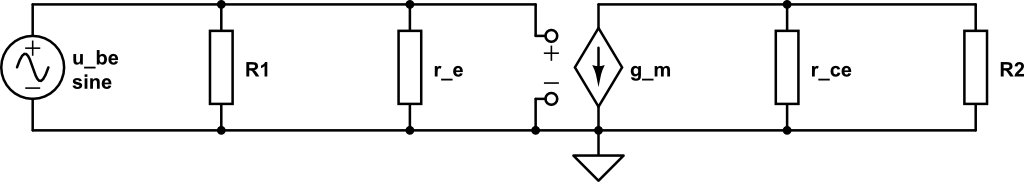
\includegraphics[width=0.8\textwidth]{resource/npn-kleinsignaal-versterker}
	\caption{Kleinsignaalmodel van NPN-spanningsversterker}
\end{figure}

De spanningsversterking is het klein-signaal model wordt gegeven door,

\begin{equation}
A_v=\frac{v_o}{v_i}
\end{equation}

\begin{equation}
v_o=-g_m\cdot u_{be}\cdot R_2'
\end{equation}
Hierin is $R_2'$ de vervangende waarde voor de parallelschakeling van $R_2$ en $r_{ce}$,
$$R_2'=\frac{R_2\cdot r_{ce}}{R_2+r_{ce}}$$

\noindent Het is meestal zo dat $r_{ce}\gg R_2$, hierdoor wordt $R_2'\approx R_2$,
$$\Rightarrow v_o=-g_m\cdot u_{be}\cdot R_2$$
Hierbij is $u_{be}=v_i$, dus de spanningsversterking is:
$$A_v=\frac{-g_m\cdot u_{be}\cdot R_2}{u_{be}}=-g_m\cdot R_2$$

\noindent De waarde van $g_m$ kan berekend worden door middel van,

\begin{equation}
g_m=\frac{I_C}{V_T}
\end{equation}
Hierin is $I_C$ de collector stroom bij het instelpunt en $V_T$ de thermische spanning van de transistor op kamertemperatuur, de waarde is ongeveer 25 mV.

$$\Rightarrow g_m=\frac{9.7\times 10^{-3}A}{25\times 10^{-3}V}= 0.39 \: S$$

Nu alle waarden berekend zijn, kan alles in de formule worden ingevuld:

$$A_v= -0.39 \: S\cdot 450 \: \Omega\approx -176 $$

\section*{Conclusie}
Het werken met de spanningsversterker circuit met behulp van een NPN-transistor geeft ons inzicht in de werking van niet-lineaire elektrische componenten. Bovendien wordt er ook inzicht verkregen in het verschil tussen groot-signaal en klein-signaal gedrag.
Om het circuit te laten werken, werden de waarden van de weerstanden bepaald door middel van de Falstad simulator en daarna door middel van een berekening.
Met het groot-signaalmodel wordt het instelpunt van de transistor bepaald. Bovendien wordt er met het instelpunt de waarde van $R_2$ berekend. Verder is de versterkingsfactor met het klein-signaalmodel te berekenen. 
Om het gedrag van de spanningsversterker circuit met behulp van een NPN-transistor te analyseren, moet er dus gebruik worden gemaakt van simulaties, groot-signaalmodel en klein-signaalmodel.

Met de opgedane kennis konden de volgende waarden worden berekend voor de spanningsversterker:
$$R_{1} = 63.8 \mathrm{k}\Omega \quad R_{2} = 450 \Omega \quad A_{v} = -176$$

\newpage
\printbibliography
\end{document}